\documentclass[a4paper,
               %boxit,        % check whether paper is inside correct margins
               %titlepage,    % separate title page
               %refpage       % separate references
               %biblatex,     % biblatex is used
               keeplastbox,   % flushend option: not to un-indent last line in References
               %nospread,     % flushend option: do not fill with whitespace to balance columns
               %hyphens,      % allow \url to hyphenate at "-" (hyphens)
               %xetex,        % use XeLaTeX to process the file
               %luatex,       % use LuaLaTeX to process the file
               ]{jacow}
%
% ONLY FOR \footnote in table/tabular
%
\usepackage{pdfpages,multirow,ragged2e} %
%
% CHANGE SEQUENCE OF GRAPHICS EXTENSION TO BE EMBEDDED
% ----------------------------------------------------
% test for XeTeX where the sequence is by default eps-> pdf, jpg, png, pdf, ...
%    and the JACoW template provides JACpic2v3.eps and JACpic2v3.jpg which
%    might generates errors, therefore PNG and JPG first
%
\makeatletter%
\ifboolexpr{bool{xetex}}{\renewcommand{\Gin@extensions}{
    .pdf,%
    .png,.jpg,.bmp,.pict,.tif,.psd,.mac,.sga,.tga,.gif,%
    .eps,.ps,%
  }}{
}
\makeatother

% CHECK FOR XeTeX/LuaTeX BEFORE DEFINING AN INPUT ENCODING
% --------------------------------------------------------
%   utf8  is default for XeTeX/LuaTeX
%   utf8  in LaTeX only realises a small portion of codes
%
\ifboolexpr{bool{xetex} or bool{luatex}} % test for XeTeX/LuaTeX
 {}                                      % input encoding is utf8 by default
 {\usepackage[utf8]{inputenc}}           % switch to utf8

\usepackage[USenglish]{babel}


%
% if BibLaTeX is used
%
\ifboolexpr{bool{jacowbiblatex}}%
 {%
  \addbibresource{jacow-test.bib}
  \addbibresource{biblatex-examples.bib}
 }{}
\listfiles

%%
%%   Lengths for the spaces in the title
%%   \setlength\titleblockstartskip{..}  %before title, default 3pt
%%   \setlength\titleblockmiddleskip{..} %between title + author, default 1em
%%   \setlength\titleblockendskip{..}    %afterauthor, default 1em

%BEAMLINE DRAWING
\usepackage{caption, subcaption}
\usepackage{tikz}
%\usepackage{etoolbox}
\usepackage{calc}

\newcommand{\correctorMagnet}[2]{
    \filldraw[blue!80] (#1,0) -- (#1-0.15, 0.7) -- (#1+0.15, 0.7);
    \filldraw[blue!80] (#1,0) -- (#1-0.15,-0.7) -- (#1+0.15,-0.7);
    
    \node[rotate=-90,anchor=west] at (#1,-0.7) {#2};
}

\newcommand{\BTV}[2]{
    \draw[ultra thick, purple] (#1,0) circle (0.4);
    \draw[ultra thick, purple] (#1,-0.3) -- (#1,0.3);
    
    \node[rotate=-90,anchor=west] at (#1,-0.7) {#2};
}

\newcommand{\cBPM}[2]{
    \draw[ultra thick, purple] (#1,0) circle (0.15);
    
    \node[rotate=-90,anchor=west] at (#1,-0.7) {#2};
}
\newcommand{\iBPM}[2]{
    \draw[ultra thick, purple] ({#1-0.25},-0.25) rectangle ({#1+0.25},+0.25);
    
    \node[rotate=-90,anchor=west] at (#1,-0.7) {#2};
}

\newcommand{\lensF}[2] {
    \pgfmathsetmacro{\lensRadius}{2};
    \pgfmathsetmacro{\lensHeight}{0.7};
    \pgfmathsetmacro{\startAngle}{asin(\lensHeight/\lensRadius)};
    
    \draw [fill=blue!15]  (#1,\lensHeight)
         arc[start angle=180-\startAngle,delta angle=2*\startAngle,radius=\lensRadius]
         arc[start angle=-\startAngle,delta angle=2*\startAngle,radius=\lensRadius]
         -- cycle; % to get a better line end

   \node[rotate=-90,anchor=west] at (#1,-0.7) {#2};
}

\newcommand{\lensD}[2] {
    \pgfmathsetmacro{\lensRadius}{2};
    \pgfmathsetmacro{\lensHeight}{0.7};
    \pgfmathsetmacro{\startAngle}{asin(\lensHeight/\lensRadius)};
    
    \draw [fill=blue!15]  (#1,\lensHeight) --
         (#1-0.2,\lensHeight)
         arc[start angle= 180+\startAngle,
             end angle  = 180-\startAngle,
             radius     = -\lensRadius] --
         (#1+0.2,-\lensHeight)
         arc[start angle=\startAngle,
             end angle=180-\startAngle,radius=\lensRadius]
         %.-- cycle; % to get a better line end

   \node[rotate=-90,anchor=west] at (#1,-0.7) {#2};
}

%TMP WHILE WRITING
%\usepackage{showframe}
\usepackage{todonotes}

\begin{document}

\title{Status of the CLEAR electron beam user facility at CERN}

\author{K. N. Sjobak\thanks{k.n.sjobak@fys.uio.no}\textsuperscript{1}, E. Adli, C. A. Lindstrom, University of Oslo, Oslo, Norway\\
  M. Bergamaschi, S. Burger, R. Corsini, A. Curcio, S. Curt, S. Doebert, W. Farabolini, D. Gamba,\\
  L. Garolfi, A. Gilardi, I. Gorgisyan, E. Granados, H. Guerin, R. Kieffer, M. Krupa, T. Lefevre,\\
  S. Mazzoni, G. McMonagle, J. Nadenau, H. Panuganti, S. Pitman, V. Rude, A. Schlogelhofer,\\
  P. K. Skowronski, M. Wendt, A. Zemanek, CERN, Geneva, Switzerland \\
  A. Lyapin, UCL, London, United Kingdom \\
  \textsuperscript{1}also at CERN, Geneva, Switzerland}

\maketitle

%
\begin{abstract}
  The CERN Linear Electron Accelerator for Research (CLEAR) is now in its second year of operation, providing a testbed for new accelerator technologies and a versatile radiation source.
  Hosting a varied experimental program, this beamline provides a flexible test facility for users both internal and external to CERN, as well as being an excellent accelerator physics training ground.
  The energy can be varied between 60 and 220 MeV, bunch length between 1 and 3 ps, bunch charge in the range 10~pC to 2 nC, and number of bunches in the range 1 to 200, at a repetition rate of 0.8 to 10 Hz.
%  X-band test capabilities have been added to the facility during this run, further enriching the range of accelerator R\&D studies performed at CLEAR.
  The status of the facility with an overview of the recent experimental results is presented.
\end{abstract}

\section{Introduction}

The CLEAR facility was built from the probe beam injector CALIFES at CTF3, reusing and upgrading the accelerator part and installing several new experiments~\cite{Gamba::CLEAR,Corsini:FirstCLEAR}.
The current beamline layout is illustrated in Fig.~\ref{fig:layout}, and a Mad-X model is available~\cite{CLEAR-MADX}.

The main purpose of CLEAR is to provide a test-bed for new accelerator technologies including beam instrumentation, plasma devices, X-band accelerating structures, and more.
Also hosted is a varied program of irradiation with electron beams, including tests for high-energy electron radio therapy techniques and validation of electronic components which must survive the radiation environment around Jupiter for the JUICE mission.
This is achieved by having a flexible, easily accessible and modifiable beam-line with a wide span of available parameters.
Typically, the tunnel is accessible every monday for experiment installation and/or modification, which makes the setup and modification experiments very easy and convenient.
In cases where more accesses have been needed (e.g.\ for irradiation), this has also been possible.
The radiation levels are generally low, which makes it possible to use a wide range of equipment.
CLEAR is also functioning as a visit point at CERN, recieving both groups and VIPs in order to teach and demostrate accelerator research facilities.
Aditionally, due to the relative simplicity of the machine and the fact that it is hard to damage through beam losses etc., it has also been used to provide training for students through programs such as JUAS.

As seen from the layout, the CLEAR machine is well equipped with diagnostics for measuring the beam parameters such as bunch charge and train length, bunch length, energy- and energy-spread, and Twiss parameters, as well as combinations thereof.
This makes it possible to quickly setup a wide variety of beams for the hosted experiments, and to cross-compare different diagnostics including prototypes.

CLEAR typically runs during normal weekdays, for 9 hours or more each day, depending on the experiment being ran and operator availability.
In 2018, there was a total of 32 weeks of operation, split over two runs with a shutdown in the summer to prepare for Xbox-1 connection to the X-band accelerating structures and for general maintainance of the facility.
Unlike the rest of the CERN accelerator complex, CLEAR will be kept running throughout Long Shutdown 2.

\begin{figure*}[t]
  \centering
  \begin{subfigure}{\textwidth}
    \centering
    %% TIKZ DRAWING OF CALIFES ELEMENTS
%% TO BE INCLUDED INTO A LATEX DOCUMENT
%% K. Sjobak, 2018

\begin{tikzpicture}

    %EOS table
    \filldraw[green] (4.9,-0.4) rectangle (2.9,0.4);
    \filldraw[green] (4.9,-0.4) rectangle (4.7,-2);
    \filldraw[green] (2.9,-0.4) rectangle (3.1,-2);
    
    %BEAM
    \draw[latex-,ultra thick] (0,0)--(15,0);
    \draw[ultra thick, dashed] (-1,0) -- (0,0);
    
    %% GUN
    \node at (15,1) {\belemsiz 0.0~m};
    
    % Gun solenoids
    \solRect{15}{0.5}{14}{0.7}
    \solRect{15}{-0.5}{14}{-0.7}
    
    \solRect{15.25}{0.5}{15}{0.7}
    \solRect{15.25}{-0.5}{15}{-0.7}
    
    % Gun cavity
    \draw[orange, ultra thick] (15,0.0) to (15,0.4)
        arc(90:180:0.15)
        arc(360:180:0.05) arc(0:180:0.15)
        arc(360:180:0.05) arc(0:180:0.15);
    \draw[orange, ultra thick] (15,0.0) to (15,-0.4)
        arc(-90:-180:0.15)
        arc(0:180:0.05) arc(0:-180:0.15)
        arc(0:180:0.05) arc(0:-180:0.15);
    
    \node[rotate=-90,anchor=west,align=left] at (15+0.25/2, -0.7)
        {\belemsiz SNH 110};
    \node[rotate=-90,anchor=west,align=left] at (14.5, -0.7)
        {\belemsiz GUN 115\\
         \belemsiz SNI 120};
    
    \correctorMagnet{13.7}{DG 130};
    \node at (13.7,1) {\belemsiz 0.32~m};
    
    %Laser mirror
    \draw[ultra thick]  ({(13.7-13)/2+13 + 0.1}, -0.1) --
                        ({(13.7-13)/2+13 - 0.1}, -0.3);
    
    %Laser
    \draw[thick,-latex,dashed]
        ({(13.7-13)/2+13},-2.25) --
        ({(13.7-13)/2+13},-0.2) -- 
        (15,0);
        
    %Laser table
    \BTV[-2.25]{14}{};
    \draw[thick, -latex, dashed]
        (13,-2.25) -- (14,-2.25);
    \node at (14.9,-2.25) {\belemsiz BTV125};
    
    \draw[ultra thick] ({(13.7-13)/2+13-0.25/2}, -2.25-0.25/2) -- 
                       ({(13.7-13)/2+13+0.25/2}, -2.25+0.25/2);
    
    %ICT 210
    \filldraw[purple] (12.95-0.1/2,-0.3) rectangle (12.95+0.1/2,0.3);
    \node[rotate=-90,anchor=west] at (12.95,-0.7) {\belemsiz ICT 210};

    \BTV{12.35}{MTV 215};
    \node at (12.35,0.7) {\belemsiz 1.81~m};
    
    \cBPM{11.8}{BPC 220}{0.15};
    \correctorMagnet{11.5}{DG 225};
    \node at (11.5,1) {\belemsiz 2.18~m};
    
    \draw[ultra thick, orange] (11.3,-0.4) rectangle (10.2,0.4);
    
    \solRect{11.3}{0.6}{10.2}{0.7}
    \solRect{11.3}{-0.6}{10.2}{-0.7}
    
    \filldraw[blue] (11.3, 0.45) rectangle (10.2,  0.55);
    \filldraw[blue] (11.3,-0.45) rectangle (10.2, -0.55);
    
    \node[rotate=-90,anchor=west, align=left] at (10.2+1.1/2,-0.7)
        {\belemsiz ACS 230\\
         \belemsiz DB 230-S\\
         \belemsiz SNG 230};
    
    \cBPM{9.9}{BPC 240}{0.15};
    \correctorMagnet{9.6}{DG 245};
    \node at (9.6,1) {\belemsiz 7.33~m};
    
    \draw[ultra thick, orange] (9.3,-0.4) rectangle (8.2,0.4);
    \node[rotate=-90,anchor=west, align=left] at (8.2+1.1/2,-0.7) {\belemsiz ACS 250\\
     \belemsiz SNG 250};

    \solRect{9.3}{0.5}{8.2}{0.7};
    \solRect{9.3}{-0.5}{8.2}{-0.7};
    
    \cBPM{7.9}{BPC 260}{0.15};
    \correctorMagnet{7.6}{DG 265};
    \node at (7.6,1) {\belemsiz 12.49~m};
    
    \draw[ultra thick, orange] (7.3,-0.4) rectangle (6.2,0.4);
    \node[rotate=-90,anchor=west] at (6.2+1.1/2,-0.7) {\belemsiz ACS 270};
    
    \cBPM{5.9}{BPC 310}{0.15};
    \correctorMagnet{5.6}{DG 320};
    \node at (5.6,1) {\belemsiz 17.70~m};
    
    \kickerHV[0]{5.125}{SDH 340}{-1}{orange};

    %\draw[ultra thick, purple] (4.15,-0.15) rectangle (3.85,0.15);
    
    \lensF{4.4}{QFD 350};
    \lensD{3.9}{QDD 355};
    \lensF{3.4}{QFD 360};
    \node at (3.9,1) {\belemsiz 18.90~m};

    
    %EOS table defined on top, to get behind the "beam"
    \draw[-latex, dashed,thick] (4.8,-2) -- (4.8,-0.2) -- (3.0,-0.2) -- (3,-2);
    %\node at (4.8,-2.25) {\belemsiz EOS laser};
    \node at (3.9,-2.25) {\textbf{Electro-Optical Sampling}};
    
    \cBPM{2.7}{BPC 380}{0.15};
    \correctorMagnet{2.4}{DG 385};
    \node at (2.4,1) {\belemsiz 19.96~m};

    \BTV{2.0}{MTV 390};
    
    %% VESPER
    
    \pgfmathsetmacro{\VesperStart}{1.5}; %Center of the dipole (X)
    \pgfmathsetmacro{\VesperAngle}{-22.0};
    %Arrow end point
    \pgfmathsetmacro{\VesperX}{-1};
    \pgfmathsetmacro{\VesperY}{(\VesperStart-\VesperX)*tan(\VesperAngle)};
    
    \pgfmathsetmacro{\VesperTabX}{-0.0};
    \pgfmathsetmacro{\VesperTabY}{(\VesperStart-\VesperTabX)*tan(\VesperAngle)};
    \filldraw[green,rotate around={-\VesperAngle:(\VesperTabX,\VesperTabY)}]
    (\VesperTabX-0.5, \VesperTabY-0.4) rectangle
    (\VesperTabX+0.5, \VesperTabY+0.4);
    %\node[rotate=-90,anchor=west] at (\VesperTabX,\VesperTabY-0.7) {\belemsiz VESPER};
    \node at (\VesperTabX+0.4, -2.5) {\textbf{VESPER}};
    
    \filldraw[gray,rotate around={-\VesperAngle:(\VesperX,\VesperY)}]
        (\VesperX-0.05, \VesperY-0.5) rectangle
        (\VesperX+0.05, \VesperY+0.5);
    
    \draw[->,ultra thick] (\VesperStart,0)--(\VesperX,\VesperY);
    
    \kickerHV[0]{\VesperStart}{BHB 400}{1}{blue};
    
    \pgfmathsetmacro{\VesperBTVaX}{0.9};
    \pgfmathsetmacro{\VesperBTVaY}{(\VesperStart-\VesperBTVaX)*tan(\VesperAngle)};
    \BTV[\VesperBTVaY]{\VesperBTVaX}{BTV420}

    % ICT 430
    \pgfmathsetmacro{\VesperICTX}{0.4};
    \pgfmathsetmacro{\VesperICTY}{(\VesperStart-\VesperICTX)*tan(\VesperAngle)};
    \filldraw[purple,rotate around={-\VesperAngle:(\VesperICTX,\VesperICTY)}]
        (\VesperICTX-0.1/2, \VesperICTY-0.3) rectangle
        (\VesperICTX+0.1/2, \VesperICTY+0.3);

    \node[rotate=-90,anchor=west] at (\VesperICTX,\VesperICTY-0.7) {\belemsiz ICT 430};

    \pgfmathsetmacro{\VesperBTVbX}{-0.5};
    \pgfmathsetmacro{\VesperBTVbY}{(\VesperStart-\VesperBTVbX)*tan(\VesperAngle)};
    \BTV[\VesperBTVbY]{\VesperBTVbX}{BTV440}
    
    
\end{tikzpicture}
    \vspace{-2.5em} % Eat the space taken by some empty nodes
    \caption{CALIFES injector}
  \end{subfigure}
  \begin{subfigure}{\textwidth}
    \centering
    \vspace{-1em}
    %% TIKZ DRAWING OF CLEAR EXPERIMENTAL BEAMLINE 1 ELEMENTS
%% TO BE INCLUDED INTO A LATEX DOCUMENT
%% K. Sjobak, 2018

\begin{tikzpicture}
    %BEAM INSTRUMENTATION TEST STAND AREA
    \filldraw[green] (11.3,-0.4) rectangle (13.7,0.4);
    \node at ({(11.3+13.7)/2},-2.25) {\textbf{BI test area}};

    %CLIC test area
    \filldraw[green] (10.9,-0.5) rectangle (6.55,0.5);
    \node at ({(10.3+7.8)/2},-2.25) {\textbf{CLIC test area}};

    %IN-AIR table
    \filldraw[green] (-0.6,-0.5) rectangle (0.5,0.5);
    \node[align=left,anchor=west] at (-0.6,1.0) {\textbf{In-Air}\\ \textbf{test area}};
    \filldraw[gray] (-0.6,-2.0) rectangle (-0.5,0.5);

    \draw[latex-,ultra thick] (0,0)--(16,0);

    \kickerHV[0]{15.8}{BHB 400}{1}{blue};

    \lensF{15.4}{QFD 510};
    \lensD{15.0}{QDD 515};
    \lensF{14.6}{QFD 520};
    \node at (15.0,1) {\belemsiz 22.86~m};

    \iBPM{14.1}{BPM 530};

    \correctorMagnet{13.8}{DJ 540};
    \node at (13.8,1) {\belemsiz 23.76~m};

    \BTV{13.3}{(BTV 545)};

    \filldraw[purple] (12.7+0.15,0.15) rectangle (12.7-0.15,-0.15);
    \node[rotate=-90,anchor=west] at (12.7,-0.7)
        {\belemsiz WCM 550};

    \correctorMagnet{12.4}{DJ 590};
    \node at (12.4,1) {\belemsiz 25.00~m};

    \iBPM{12.0} {BPM 595}; %{BPM 560};

    \filldraw[purple] (11.5+0.15,0.15) rectangle (11.5-0.15,-0.15);
    \node[rotate=-90,anchor=west] at (11.5,-0.7)
        {\belemsiz BPR 600};

    %\cBPM{11.1}{BPC 565}{0.15};
    \cBPM{11.1}{BPC 610}{0.15};

    \BTV{10.5}{BTV 620};
    \node at (10.5,1) {\belemsiz 25.85~m};

    \draw[ultra thick, orange] (10.1,-0.4) rectangle (9.7,0.4);
    \node[rotate=-90,anchor=west] at (9.9,-0.7)
        {\belemsiz ACS 640};

    \draw[ultra thick, orange] (9.6,-0.4) rectangle (9.2,0.4);
    \filldraw[purple] (9.55,-0.5) rectangle (9.5,0.5);
    \node[rotate=-90,anchor=west,align=left] at (9.4,-0.7)
        {\belemsiz WFM 645\\[-0.5em]
         \belemsiz ACS 650};

    \cBPM{9.0}{BPC 660}{0.1};
    \cBPM{8.7}{BPC 670}{0.1};
    \cBPM{8.4}{BPC 680}{0.1};
    \cBPM{8.1}{BPC 690}{0.1};

    \correctorMagnet{7.8}{DJ 710};
    \node at (7.8,1) {\belemsiz 29.32~m};

    \cBPM{7.5}{BPC 720}{0.15};

    \BTV{6.9}{BTV 730};

    \lensF{6.3}{QFD 760};
    \lensD{5.9}{QDD 765};
    \lensF{5.5}{QFD 770};
    \node at (5.9,0.9) {\belemsiz 30.62~m};


    \correctorMagnet{5.1}{DJ 780};
    \node at (5.1,1.15) {\belemsiz 31.66~m};

    \cBPM{4.8}{BPC 790}{0.15};

    \lensF[green]{4.3}{PLC 800\\[-0.5em]
             \belemsiz BTV 800\\[-0.5em]
             \belemsiz BTV 805};
    \node at (4.3,-2.25) {\textbf{Plasma lens}};
    \node at (4.3,0.9) {\belemsiz 32.26~m};


    \BTV{3.8}{BTV 810};

    \iBPM{3.2}{BPM 820};

    \correctorMagnet{2.8}{DJ 840};
    \node at (2.8,1) {\belemsiz 33.38~m};

    \lensD{2.3}{QDD 870};
    \lensF{1.9}{QFD 880};

    %% IN-AIR SPECTROMETER

    \pgfmathsetmacro{\InAirStart}{1.5};
    \pgfmathsetmacro{\InAirAngle}{-22.0};
    \pgfmathsetmacro{\InAirY}{(\InAirStart+0.6)*tan(\InAirAngle)};

    \draw[-latex,ultra thick] (\InAirStart,0)--(-0.6,\InAirY);
    \kickerHV[0]{\InAirStart}{BHB 900}{1}{blue};
    \node at (\InAirStart,1) {\belemsiz 35.03~m};


    \pgfmathsetmacro{\InAirBTVaX}{0.0};
    \pgfmathsetmacro{\InAirBTVaY}{(\InAirStart-\InAirBTVaX)*tan(\InAirAngle)};
    \BTV[\InAirBTVaY]{\InAirBTVaX}{BTV930};

    \pgfmathsetmacro{\InAirBPMx}{0.5};
    \pgfmathsetmacro{\InAirBPMy}{(\InAirStart-\InAirBPMx)*tan(\InAirAngle)};
    \iBPM[\InAirBPMy]{\InAirBPMx}{BPM920};

    %% IN-AIR TABLE INSTRUMENTATION
    \BTV{0.9}{BTV 910};
%    \node[anchor=south] at (0.9,0.3) {\belemsiz BTV 910};

    %ICT 210
    \filldraw[purple] (0.5-0.1/2,-0.3) rectangle (0.5+0.1/2,0.3);
    \node[anchor=south] at (0.5,0.3) {\belemsiz ICT 915};

\end{tikzpicture}
    \vspace{-0.5em}
    \caption{Experimental beamline
      (continues after CALIFES, shown above)}
  \end{subfigure}
  \begin{subfigure}{\textwidth}
    \centering
    \vspace{-0.5em}
    %% TIKZ DRAWING OF CALIFES ELEMENTS
%% TO BE INCLUDED INTO A LATEX DOCUMENT
%% K. Sjobak, 2018

\begin{tikzpicture}
    
    \solRect{-3.5}{0.5}{-3.2}{0.7};
    \solRect{-3.5}{-0.5}{-3.2}{-0.7};
    \draw[->,ultra thick] (-3.2,0)--(-3.8,0);
    \node[align=left,anchor=west] at (-3.2,0) {Solenoid};

    \kickerHV[0]{-1.5}{}{1}{blue};
    \node[align=left,anchor=west] at (-1.3,0) {Dipole};

    \correctorMagnet{0.0}{};
    \node[align=left,anchor=west] at (0.2,0) {Corrector\\ magnet};
    
    \lensF{2.0}{};
    \lensD{2.5}{};
    \node[align=left,anchor=west] at (2.75,0) {Focusing /\\ defocusing\\ magnet};

    \BTV[0.5]{5}{};
    \node[align=left,anchor=west] at (5.3,0.5) {BTV screen};
    
    \cBPM[-0.05]{5}{};
    \node[align=left,anchor=west] at (5.3,-0.05) {Cavity BPM};
    
    \iBPM[-0.5]{5}{};
    \node[align=left,anchor=west] at (5.3,-0.5) {Inductive BPM};

\end{tikzpicture}


\begin{tikzpicture}

    \filldraw[blue] (-2,-1.5) rectangle (0,-1.);
    \node at (-1,-1.25) {\textbf{Magnet}};

    \filldraw[orange] (1,-1.5) rectangle (3,-1.);
    \node at (2,-1.25) {\textbf{RF element}};

    \filldraw[purple] (4,-1.5) rectangle (6,-1.);
    \node at (5,-1.25) {\textbf{Instrument}};

    \filldraw[green] (7,-1.5) rectangle (9,-1.);
    \node at (8,-1.25) {\textbf{Experiment}};

\end{tikzpicture}
    \vspace{-2em} % Eat the space taken by some empty nodes
    \caption{Symbols}
  \end{subfigure}
  \caption{Overview of the elements directly interacting with the beam at CLEAR beamline, and the location of the experimental stations as of April 2019. Element positions indicate the middle of each element, rounded to the nearest cm.}
  \label{fig:layout}
\end{figure*}

\section{Operation and Performance}

\begin{table}[t]
  \centering
  \caption{Typical beam parameters.}
  \label{tab:beamparameters}
  \begin{tabular}{c c}
    \toprule
    \textbf{Parameter} & \textbf{Value} \\
    \midrule
    Beam energy       &  60~MeV -- 220~MeV\\
    Bunch charge      &  10~pC  -- 1.5~nC \\
    Bunch length      &   1~ps  -- 3~ps \\
    Bunch frequency   &   1.5~GHz \\
    RF frequency      &   3.0~GHz \\
    Number of bunches &   1 -- 200 \\
    Beam repetition rate   & 1/(1.2~s) -- 10~Hz \\
    RMS $\epsilon_N$ at QFD350 entrance & 1~$\mu$m--15~$\mu$m\\
    Typ. $\beta$ at QFD350 entrance & 5 -- 15~m \\
    Typ. $\alpha$ at QFD350 entrance & -1 to +1 \\
    \bottomrule
  \end{tabular}
\end{table}

While CLEAR can provide a wide range of beams, the typical beam parameters are listed in Table~\ref{tab:beamparameters}.
This refers to a beam produced using the photocathode laser, which is the normally used arrangement.
Here the number of bunches, the bunch charge, and the train repetition rate is controlled via the laser parameters~\cite{LucaGun,BrossardGun}.
Single laser pulses can be picked through a system with two fast pockel cells.
Recently, the control of this system has been significantly improved, by changing the actuators controlling the mirror from picomotors to stepping motors.
This means that the beam position is easily repeatable.
Furthermore, an adjustable telescope has been added which allows to change the focus of the laser on the photocathode, and thus increasing the laser spotsize to avoid saturation when working with high-charge bunches.
Finally, the laser stability has been improved, resulting in much less pointing jitter and higher beam quality.
A double-pulse setup has been created, making it possible to double up each pulse of the laser through an optical delay line.
This will make it possible to inject two bunches into the same RF bucket, with adjustable distance.

Additionally it is also possible to collect and accelerate the dark current produced by the gun in order to make a long train with sub-pC bunch charge; this is sometimes used for radiation hardness testing of electronics.

For the RF system, the connection of the MKS31 klystron to the SDH~340 RF deflector was completed, as was the upgrades of the modulators for the other klystrons.
This has helped RF system reliability, as well as brought the control system in line with current standards.

%FESA upgrades

On the beam-line, two quadrupoles QDD870 and QFD880 have been installed in order to provide a narrow beam-spot into the In-Air test area and to measure the beam emittance after the plasma lens using the quadrupole tuning method.
Furthermore, the corrector 590 was moved upstream by 460~mm, in order to have the BPMs now named 595 and 610 installed after the orbit bump made by corrector 540 and 590.
The alignment of the quadrupoles and the accelerating structures has generally been verified and corrected by the survey group.
The beam-pipe passing through the quadrupoles were then aligned relatively to the magnets using a conical clamp.
Based on the alignment of the quadrupole beam-pipes and a point provided on the final dump, the rest of the machine was aligned using a laser passed through the center of the beam pipe from one end to the other.
This reduced beam losses, and reduced the time needed to setup a beam, especially for the experiments located after the CLIC test area.

The vacuum control system is also under consolidation, moving all the ion pump controllers into the same building and updating the interlock system and control system.

The inductive BPMs, which originally were installed on the CTF3 drive beam, have been modified to work with the lower bunch charges of CLEAR and are currently in the process of being fully comissioned.

One issue that was found and corrected during the shutdown 2018/2019 winter shut-down was the calibration of the beam charge monitors.
These devices are Integrating Current Transformers~\cite{BergozICT}, and 3 such devices are installed in the CLEAR linac and used as the main beam charge monitoring devices.
They are connected to an integrating circuit in the gallery, which computes the total charge within a time-window, and creates a long voltage pulse at a level proportional to the charge.
The error was due to the conversion of this voltage to a charge reading, resulting in a measured charge exactly 10 times smaller than the actual.
The wrongly reported charge was noticed by experiments~\cite{MarisTali:E-SEU,Antonio::IEEE-Kicks}, and then confirmed by using the calibration standard normally used to test the inductive BPMs.

%\todo[inline]{In general... stability etc.}

\section{Overview of experimental program}

There are a number of experimental stations along the beam line, as marked in green on Figure~\ref{fig:layout}.
Some of these host permanently installed experiments like the CLIC test area and the Plasma Lens Experiment.
Others are used for more temporary experiments, such as VESPER, which is used to host various irradiation tests; or the In-air test area which is used for tests of THz generation, as well as protoype advanced beam instrumentation for beam position and bunch length measurement.

Some experiments are also using the whole or parts of the machine itself as an experimental facility, such as beam dynamics studies of the RF-gun, or measurements of magnetic stray field spectra in beam facilities to benchmark models for CLIC.

\subsection{VESPER electronic component irradiation}
The VESPER test area is mainly used for irradiation of electronic components, in order to verify their functionality in radiation environments.
The main user here has been the JUICE mission~\cite{MarisTali:E-SEU,MarisTali:E-SEL,RubenAlia::CLEARrev}, however tests of components for ATLAS have also been done.
These experiments have sometimes been run in automated mode over nights and weekends, requiring only a low-intensity dark current beam.

\subsection{Medical irradiation tests}
% \begin{figure}
%   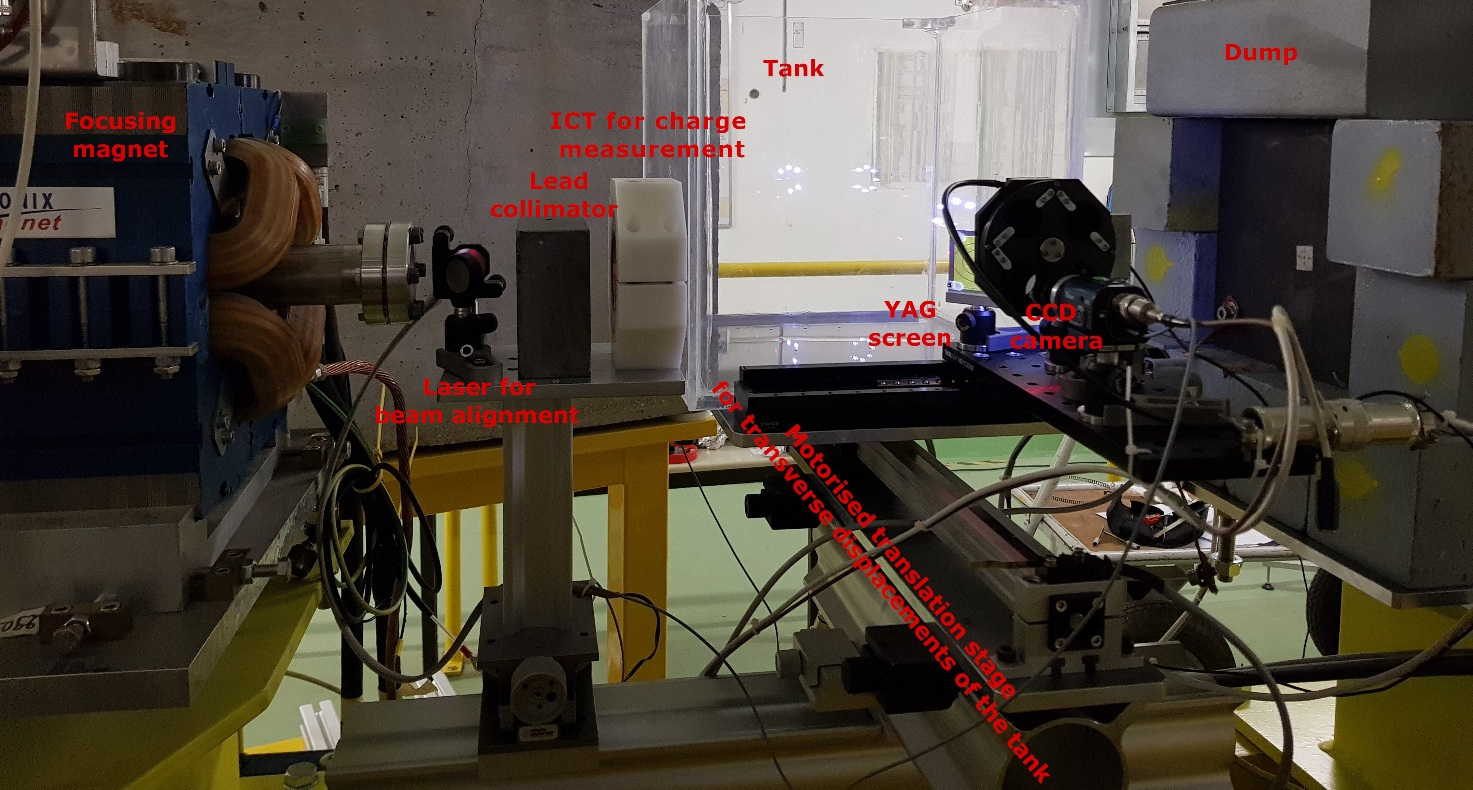
\includegraphics[width=\columnwidth]{fig/MedicalInstall_crop.jpg}
%   \caption{Temporarilly installed irradiation test.}
% \end{figure}
Several tests of medical irradiation have been done at CLEAR~\cite{Wilfrid::CLEARrev}, both at VESPER, and at a temporarilly constructed target station immediately after QFD~520.
This was done to test the effects of FLASH irradiation~\cite{FLASH2017} in biological samples, calibrate dosimeters for ultra-short VHEE pulses, and the use of steeply converging energetic electron beams for conformal irradiation.

\subsection{CLIC module tests}
The CLIC test area contains two CLIC-type accelerating structures with integrated damping of long range wake fields~\cite{Grudiev:TD26}, mounted on a movable girder~\cite{Durand-mover::AccelAlign12,Sosin-mover::IPAC12}.
These structures were originally installed as part of the two-beam test stand, and are currently not connected to an RF power source.
They are currently used for measurements of short-range wake field kicks~\cite{Antonio::IEEE-Kicks} and Wake field monitors~\cite{KyrreSjobak::CLICWS19}, both important for the feasibility of reaching CLIC performance goals~\cite{CLIC-CDR,CLIC-PIP}.

\todo[inline]{say someting about the experimental procedures}

Furthermore, four CLIC-type prototype cavity BPMs are installed just downstream of the accelerating structures.
Here, the BPMs themselves as well as the electronics are currently being tested, with initial tests indicating that a more robust in-tunnel electronics is needed.
This is currently under development~\cite{AlexejLyapin::CLICWS19} and we expect to test it in 2019.

\subsection{Plasma lens}
%\begin{figure}
%    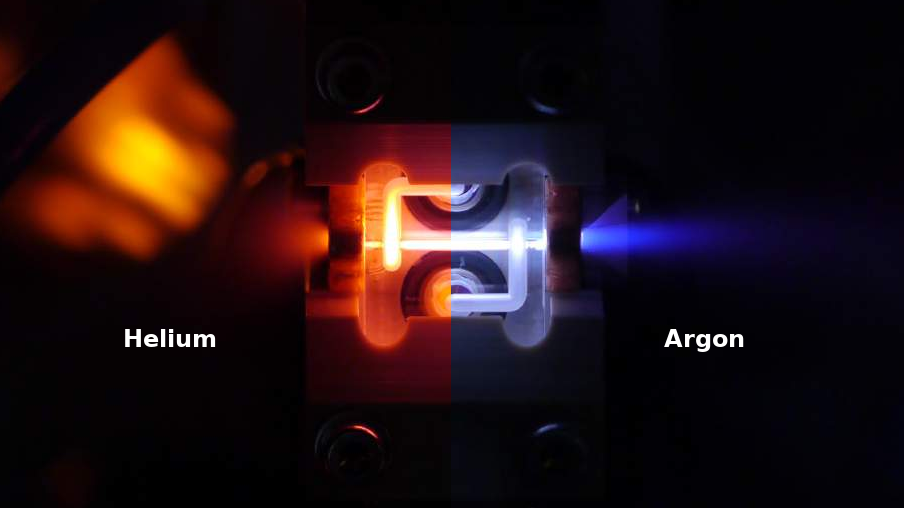
\includegraphics[width=\columnwidth]{fig/HeAr.png}
%    \caption{Discharges in the CLEAR plasma lens experiment.}
%\end{figure}

Active plasma lenses is a technology enabling strongly focusing magnetic lenses for charged particle beams.
Different from magnetic quadrupoles, they focus the beam radially, i.e.\ in both the horizontal and vertical plane.
This removes the need for using multiple lenses to control the beam size, and may have important applications for XXXX\todo{...}.

The CLEAR plasma lens experiment has focused on showing emittance preservation and uniformity of the focusing gradient in different gasses.
In 2018 the effect of the gas atomic weight on the development of focusing nonlinearities was demonstrated, showing that a linear focusing field and preservation of emittance can be achieved through the use of Argon gas~\cite{CarlPRL}.

\todo[inline]{mini-OTR and window valve, spot sizes reached}

\subsection{In-air test stand}

At the end of the CLEAR experimental beamline is the In-Air test stand, which is an optical table at the end of the beam line, before the dump.
This is used for experiments in Terrahertz generation~\cite{CurcioPRAB} and tests of novel beam instrumentation for measuring beam position and bunch length~\cite{Thibaut::CLEARrev}.

\section{Near-term plans}

An upgrade of the current analog BTV beam observation system, which is heavily used for both beam setup and experiments, is under testing.
As a test, a Bassler Gig-E camera has been installed at BTV 620, sharing the light from that camera using an optical beam splitting mirror.
This has shown that such cameras can function in the environment at CLEAR.

As mentioned earlier, the waveguide line for connecting the Xbox-1 X-band RF station\todo{cite} to the CLIC accelerating super-structure has been built\todo{cite}, however due to technical issues with the klystron it is not yet connected.
We expect this to happen during 2019, and will enable experiments \todo{...} as well as increased energy for the last part of the experimental beamline.

Furthermore, a second experimental beam line is being planned, to be connected at the location of the VESPER spectrometer bending magnet shown in Figure \ref{fig:layout}.
This will enable the installation of more experiments, as well as simplifying experiments needing a strongly focused beam in air, without needing to dismatle parts of the beam-line as done in 2018.

CITE~\cite{Roberto::CLEARrev}

\section{Conclusion}

\ldots

\begin{thebibliography}{99}
\bibitem{Gamba::CLEAR} D. Gamba et al., “The CLEAR user facility at CERN,” Nuclear Instruments and Methods in Physics Research Section A: Accelerators, Spectrometers, Detectors and Associated Equipment, Dec. 2017.

\bibitem{Corsini:FirstCLEAR} R. Corsini et al., “First Experiments at the CLEAR user facility,” in Procedings of IPAC2018, Vancouver, BC, Canada, 2018, p. 4.

\bibitem{CLEAR-MADX} \url{https://gitlab.cern.ch/CLEAR/CLEARLattice}.

\bibitem{BergozICT} Bergoz Instrumentation, “Integrating Current Transformer User’s Manual.”.

\bibitem{LucaGun} L. Garolfi et al., “Beam Dynamics Studies and Instrumentation Tests for Bunch Length Measurements at CLEAR,” in Proceedings of the 29\textsuperscript{th} Linear Accelerator Conf., 2018, vol. LINAC2018, pp. 4 pages.

\bibitem{BrossardGun} J. Brossard, M. Desmons, B. M. Mercier, C. P. Prevost, and R. Roux, “Construction of the Probe Beam Photo-injector of CTF3,” 2006, p. 3.

\bibitem{MarisTali:E-SEU} M. Tali et al., “Mechanisms of Electron-Induced Single-Event Upsets in Medical and Experimental Linacs,” IEEE Transactions on Nuclear Science, vol. 65, no. 8, pp. 1715–1723, Aug. 2018.

\bibitem{Antonio::IEEE-Kicks} P. Arpaia, R. Corsini, A. Gilardi, and K. N. Sjobak, “Beam–based alignment of the CLIC high-gradient X-Band accelerating structure using beam-screen,” in proceedings of the International Instrumentation and Measurement Technology Conference, May 2019.

\bibitem{MarisTali:E-SEL} M. Tali et al., “Mechanisms of Electron-Induced Single-Event Latchup,” IEEE Transactions on Nuclear Science, vol. 66, no. 1, pp. 437–443, Jan. 2019.

\bibitem{RubenAlia::CLEARrev} Rubén García Alía, Maris Tali, ``VESPER and R2E activities,'' presetned at the CLEAR review 2019. \url{https://indico.cern.ch/event/781404/contributions/3304093/}

\bibitem{Wilfrid::CLEARrev} W. Farabolini, R. Corsini, D. Gamba, K.N. Sjobak, L. Garolfi, A. Gilardi, E. Senes, A. Lagzda, R. Jones, K. Kokurewicz, E. Brunetti, A. Subiel, M. McManus, F. Romano, M.-C. Vozerin, P. Goncalves, C. Bailat, ``VHEE and FLASH Medical Studies,'', presented at the CLEAR review 2019. \url{https://indico.cern.ch/event/781404/contributions/3304095/}

\bibitem{FLASH2017} P. Montay-Gruel et al., “Irradiation in a flash: Unique sparing of memory in mice after whole brain irradiation with dose rates above 100 Gy/s,” Radiotherapy and Oncology, vol. 124, no. 3, pp. 365–369, Sep. 2017.

\bibitem{Grudiev:TD26} A. Grudiev and W. Wuensch, “Design of the CLIC Main Linac Accelerating Structure for CLIC Conceptual Design Report,” presented at the LINAC’10, Tsukuba, Japan.

\bibitem{Durand-mover::AccelAlign12} Mainaud Durand, H, Anastasopoulos, M, Griffet, S, Griffet, S, Rude, V, and Sosin, M, “VALIDATION OF THE CLIC ALIGNMENT STRATEGY ON SHORT RANGE,” presented at the International Workshops on Accelerator Alignment, Fermilab, Batavia, IL, USA, 2012.

\bibitem{Sosin-mover::IPAC12} M. Sosin et al., “Issues and Feasibility Demonstration of Positioning Closed Loop Control for the CLIC Supporting System Using a Test Mock-up with Five Degrees of Freedom,” presented at the IPAC’12, 2012.

\bibitem{KyrreSjobak::CLICWS19} Kyrre Sjobak, ``Tests of Wakefield Monitors (WFMs) at CLEAR'', presented at CLIC workshop 2019. \url{https://indico.cern.ch/event/753671/contributions/3285765/}

\bibitem{CLIC-CDR} A Multi-TeV Linear Collider Based on CLIC Technology: CLIC Conceptual Design Report. 2012.

\bibitem{CLIC-PIP} CERN, “The Compact Linear Collider (CLIC) – Project Implementation Plan - CERN Yellow Reports: Monographs, Vol 4 (2018),” CERN, Jan. 2019.

\bibitem{AlexejLyapin::CLICWS19} A. Lyapin, M. Cargnelutti, M. Wendt, ``Cavity BPM at CLEAR'', presented at CLIC workshop 2019. \url{https://indico.cern.ch/event/753671/contributions/3272592/}

\bibitem{CarlPRL} C. A. Lindstrøm et al., “Emittance Preservation in an Aberration-Free Active Plasma Lens,” Phys. Rev. Lett., vol. 121, no. 19, p. 194801, Nov. 2018.

\bibitem{Thibaut::CLEARrev} T. Lefevre, ``Diagnostics and THz activities'', presented at the CLEAR review 2019. \url{https://indico.cern.ch/event/781404/contributions/3304102/}

\bibitem{CurcioPRAB} A. Curcio et al., “Beam-based sub-THz source at the CERN linac electron accelerator for research facility,” Physical Review Accelerators and Beams, vol. 22, no. 2, Feb. 2019.

\bibitem{Roberto::CLEARrev} R. Corsini, ``CLEAR upgrades -- evolution -- future programs'', presented at the CLEAR review 2019. \url{https://indico.cern.ch/event/781404/contributions/3304104/}

\end{thebibliography}

\end{document}
